\section{从电流元受力到导线的合力}
已知电流产生的磁场以后，接下来要区分“产生磁场的电流”和“受到磁力的电流”。对理想细导线元，外磁场给予的力为
\begin{equation}\dd\bm F=I\dd\bm l\times\bm B_{\rm ext}.\end{equation}
这里的场不包括所取电流元本身的奇异自场。计算两条导线之间的相互作用时，一条产生场，另一条受力；讨论完整导线的自应力则需要更细致地分离各段，不能把长直线自己的场直接放入自身的 $BIl$ 中。


若外场均匀，$\bm B$ 可提出积分号，得到 $\bm F=I(\bm r_B-\bm r_A)\times\bm B$。弯曲导线的合力因此只与两端点有关；端点连线是有向位移，不是导线的实际长度。闭合线圈的端点重合，合力为零，却仍可能受到力偶。若外场随位置变化，$\bm B$ 不能提出积分号，闭合回路也可能有非零合力。


受力图中应把实际电流方向与参考正方向分开。若最后算得电流为负，磁力方向也要随之反向。对运动导体，磁力还可能反馈改变运动状态；静磁平衡题虽然不要求完整的电磁暂态，仍要说明给定电流由外部电源维持，或在短脉冲期间近似不变。

\fig{fig:mg2:k:force}{均匀场中弯曲导线的端点位移}{\begin{tikzpicture}[scale=.88]
\draw[world](0,0)to[bend left=50](2,1)to[bend right=30](4,0);\node[left]at(0,0){$A$};\node[right]at(4,0){$B$};\draw[flow](0,-.7)--(4,-.7)node[midway,below]{$\bm r_B-\bm r_A$};\node at(2,2){$\odot B$};
\end{tikzpicture}}

图\ref{fig:mg2:k:force}的直箭头是端点有向位移，曲线才是实际导线。均匀场允许将 $\bm B$提出积分号，使各电流元只留下 $\int\dd\bm l=\bm r_B-\bm r_A$；若场不均匀，便不能用该直线代替整条曲线积分。


\section{平行电流的作用与电荷力的比较}
两条相距 $d$ 的长直导线中，一条电流 $I_1$ 在另一条所在处产生场 $\mu_0I_1/(2\pi d)$。取第二条长度 $l$，受力大小为 $\mu_0I_1I_2l/(2\pi d)$。同向电流相吸、反向电流相斥，结论应由电流与场的叉乘得到，不能把“电荷同号相斥”的判断替代为电流相互作用。


有些输电问题中，导线还带有表面净电荷。理想细长平行线的电荷力每单位长度为 $\lambda_1\lambda_2/(2\pi\varepsilon_0d)$，方向由电荷正负决定。若两线带异号电荷并有反向电流，电荷力相吸、磁力相斥，二者可能恰好平衡。电压与单位长度电荷之间的关系需要由给定的单位长度电容建立；把电压直接当作电荷密度会造成量纲错误。


电流使导线受到机械力，能量由维持电流的外部装置供给。轨道导体、线圈与导磁物之间的加速过程都需要把电源、磁场和机械运动联系起来；用静磁公式求瞬时力，只是其中的受力部分。脉冲式线圈加速还涉及自感和切换，相关时间过程在电磁感应专题中展开。

\fig{fig:mg2:k:parallel}{先由另一根导线的场确定磁力，再与净电荷的电力分别比较}{\begin{tikzpicture}

\node at(-1.5,0){$\odot I_1$};\node at(1.5,0){$\odot I_2$};\draw[->,blue,thick](1.5,.3)--(1.5,1.6)node[above]{$\bm B_1$};
\draw[force](1.2,0)--(.1,0)node[midway,below]{$\bm F_2$};\draw[force](-1.2,0)--(-.1,0)node[midway,above]{$\bm F_1$};
\draw[dim](-1.5,-1)--(1.5,-1)node[midway,below]{$d$};\node at(0,2.3){同向电流相吸};
\begin{scope}[xshift=6.4cm]
\node[align=center]at(-1.5,0){$\odot I$\\$+\lambda$};\node[align=center]at(1.5,0){$\otimes I$\\$-\lambda$};
\draw[->,red,thick](1.2,.7)--(.1,.7)node[midway,above]{$F_e$};\draw[->,blue,thick](1.8,-.7)--(2.8,-.7)node[midway,below]{$F_m$};
\node at(0,2.3){反向电流、异号电荷};\node at(.3,-1.6){电力向内，磁力向外};
\end{scope}

\end{tikzpicture}}
图\ref{fig:mg2:k:parallel}左图在第二根导线处画的是第一根产生的场 $\bm B_1$；再由第二根的电流方向作叉乘，得到向第一根的磁力。右图则对同一根导线同时保留电力与磁力。以每单位长度表示，两种力的大小之比为

\[
 \frac{f_m}{f_e}=\frac{\mu_0\varepsilon_0 I^2}{\lambda^2}
\]
（两根的电流大小同为 $I$、净线电荷大小同为 $\lambda$）。这里 $I$ 与 $\lambda$ 是不同物理量；金属中维持电流的载流子数量不等于导线的净电荷量，所以不能直接将二者的比值都解释为同一个漂移速度。



\section{两层电流的磁压力}
设两无限平行薄电流层电流密度大小都为 $K$、方向相反。单层在任一侧产生的磁感应强度大小为 $\mu_0K/2$，两层之间叠加成 $B=\mu_0K$，外侧相消。取一层面积 $A$ 的小片，片上电流总量按 $K$ 乘以横向长度计算。受力必须使用另一层产生的场，故单位面积受力为

\[
p=K\frac{\mu_0K}{2}=\frac{B^2}{2\mu_0}.
\]
反向电流互斥，因而两层受到朝外的力。若误把层间总场 $B$ 全部作为外场，就会重复计入该层自己的贡献，使结果扩大一倍。把两层各自的场先画出，再作叠加，能同时确定区域场和受力方向。


式中 $B^2/(2\mu_0)$ 的量纲为能量密度，也等于压强量纲。这种对应有助于检验数值，但并不表示任意场的边界受力都可直接套用同一个标量公式。磁场相对于表面的法向、切向分量不同，磁应力的方向也不同。此处的结论依赖于场沿层面、两侧一侧有场而另一侧为零的特定构型。


对于有限宽板，边缘附近的场会弯曲，均匀压力近似只适用于离边缘较远的中央部分。计算总力可先以 $pA$ 为主要贡献，再按尺寸和间距评估边缘修正；不能用无限模型推导后又声称有限板每一点都严格具有同样压力。

\fig{fig:mg2:k:pressure}{反向电流层的场叠加与相互排斥}{\begin{tikzpicture}[scale=.88]
\draw[world](-2,-1)--(2,-1) (-2,1)--(2,1);\node[right]at(2,1){$\odot K$};\node[right]at(2,-1){$\otimes K$};\draw[flow](-1,0)--(1,0)node[midway,below]{$B=\mu_0K$};\draw[force](0,1)--(0,2)node[above]{$p$};\draw[force](0,-1)--(0,-2)node[below]{$p$};\node at(-2.7,1.7){$B=0$};\node at(-2.7,-1.7){$B=0$};
\end{tikzpicture}}

图\ref{fig:mg2:k:pressure}的层间总场由两层各贡献一半。计算上层受力时只保留下层的场，计算下层时反之，所以每层磁压力为 $K(\mu_0K/2)$。向外的力箭头与反向电流互斥相符，不能再用总场重复算自身贡献。


\section{磁力的分解、支持力与摩擦阈值}
棒放在导轨上时，磁力一般既可沿轨道推动，也可改变支持力。摩擦力上限是 $\mu N$，只有在支持力确为 $mg$ 时才能写成 $\mu mg$。因此，寻找最小磁场时应把磁场方向也作为待定变量，同时检查接触条件 $N\ge0$。


以水平轨道上的直棒为例，若长度方向与观察平面垂直，允许磁力在平面内斜向上，设磁力与水平夹角为 $\alpha$。则临界滑动要求
\[
IlB\cos\alpha=\mu(mg-IlB\sin\alpha).
\]
把 $B$ 解出后，要让分母 $\cos\alpha+\mu\sin\alpha$ 最大。由 $\cos\alpha+\mu\sin\alpha=\sqrt{1+\mu^2}\cos(\alpha-\arctan\mu)$，最优方向自然确定。这个优化既利用水平分量，又利用减小支持力的竖直分量；达到最优值后还需代回检查棒没有先离开导轨。


在斜面上，重力与磁力都应先按切向、法向分解，再决定摩擦方向。若题目只问维持静止所需条件，静摩擦并不自动取最大值；只有临界滑动时才能把不等式写成等式。计算所得“平衡电流”还可能对应失去接触或另一方向滑动，必须回到受力图判断。

\fig{fig:mg2:k:contact}{磁力既推动导棒，也改变支持力}{\begin{tikzpicture}[scale=.88]
\draw[world](-2,-.2)--(2,-.2);\fill(0,0)circle(3pt);\draw[force](0,0)--(2,1)node[right]{$\bm F_B$};\draw[force](0,0)--(0,1.8)node[above]{$N$};\draw[force](0,0)--(0,-1.7)node[below]{$mg$};\draw[force](0,0)--(-1.5,0)node[left]{$f$};\node at(1,.15){$\alpha$};
\end{tikzpicture}}

图\ref{fig:mg2:k:contact}中的磁力竖直分量减小支持力，水平分量克服摩擦。两分量共同进入临界式；最优磁场方向确定后，还须代回检查 $N\ge0$及所需摩擦方向，否则可能把已脱离导轨的状态当作临界滑动。


\section{磁矩、力矩与转动平衡}
矩形线圈在均匀磁场中两组对边所受力合成力偶，计算力臂后得到 $\bm\tau=\bm m\times\bm B$。平面线圈的磁矩为 $\bm m=NI S\bm n$，法线方向与电流成右手关系。夹角 $\theta$ 是磁矩与场的夹角；若题目给的是线圈平面与场的夹角，必须先换成余角。


力矩方向由磁矩与外场的叉乘决定；下面先从任意平面回路的分布力推导，再讨论转动能量与稳定性。
\fig{fig:mg2:k:torque}{角度从线圈法线量到外场；向纸内的力矩使正夹角减小}{\begin{tikzpicture}

\draw[flow,blue](0,0)--(3.5,0)node[right]{$\bm B$};\draw[flow,red](0,0)--(2,2)node[above]{$\bm m=NIS\bm n$};
\draw[very thick](-1.1,1.1)--(1.1,-1.1);\node[left,align=center]at(-1.2,1.1){线圈平面\\侧视};\draw[dim](.7,0)arc(0:45:.7)node[midway,right]{$\theta$};
\draw(-.15,.15)--(0,.3)--(.15,.15);\node at(2.5,-1){$\otimes\bm\tau$};\node at(1,-1.9){$\tau_\theta=-mB\sin\theta$};

\end{tikzpicture}}

图\ref{fig:mg2:k:torque}的 $\theta$在磁矩与外场之间量取，而磁矩垂直线圈平面。增大 $\theta$的广义力矩为 $-mB\sin\theta$，故平行方向受到回复作用；不能把线圈平面与场的角直接代入同一个正弦式。


\subsection{非均匀场中的力与选轴}
对尺寸远小于场变化尺度的磁偶极子，若磁矩方向被约束不变，机械力为 $\bm F=\nabla(\bm m\cdot\bm B)$。方向沿轴且只随轴向坐标改变时，化为 $F_z=m\,\dd B/\dd z$。这个公式含有场的梯度；单靠场值大，不能推出吸引力一定大。


线圈尺寸不可忽略时，应逐边积分。总力矩还必须说明关于哪个点或哪条轴。某条边的合力虽可集中在其几何中点，但前提是这条边上的场分布足够对称；场沿边不均匀时，应把微元力矩 $\bm r\times\dd\bm F$ 先积分。两个竖直载流边在长直导线的场中受径向力，绕自身中轴的力矩取决于线圈平面相对径向的位置，只给某一条边离导线的距离通常不足以完全确定几何关系。

\section{从分布力得到平面电流的力矩}
磁矩公式可以由每一小段导线的力直接建立。先把任意形状的平面闭合回路放在 $xy$ 平面，规定电流从 $+z$ 看为逆时针，取外场 $\bm B=B\bm e_x$。电流元 $I(\dd x\bm e_x+\dd y\bm e_y)$ 受到的力为 $\dd\bm F=-IB\dd y\bm e_z$，其关于原点的力矩是

\[
\dd\bm\tau=IB(-y\dd y\bm e_x+x\dd y\bm e_y).
\]
第一项是全微分，$\oint y\dd y=\oint\dd(y^2/2)=0$。
第二项可按水平窄条理解：在逆时针边界右侧，$\dd y>0$，左侧绕行时 $\dd y<0$，故
\[
 \oint x\dd y=\int_{y_{\min}}^{y_{\max}}
 [x_{\rm right}(y)-x_{\rm left}(y)]\dd y=S.
\]
若一条水平线与边界有多次交会，就把各段条带宽度相加；同样得到有向面积。因此 $\tau_y=IBS$，其余分量为零。把坐标系转回任意方向，就得到 $\bm\tau=\bm m\times\bm B$，其中 $\bm m=IS\bm n$，$\bm n$ 由电流右手定则确定。


这个推导没有要求回路是圆形或矩形。若回路有凹入部分，面积仍取整个有向面积；若有多匝，需先判断每匝面积和电流方向，再作矢量和。均匀场中闭合回路的合力为零，所以更换取矩点不会改变总力矩。非均匀场中合力可能不为零，换轴时必须加上新旧原点位移与合力的叉积，不能仍把力矩当作与轴无关。


磁矩提供的是回路远场和均匀外场力矩的简洁表达。用它分析近距离导线之间的相互作用时，场在回路范围内可能明显变化，应回到各边积分。能否作偶极近似，决定于回路尺寸相对于外场变化尺度，而不只决定于回路电流是否很小。

\fig{fig:mg2:k:plane-torque}{平面电流元与力矩方向}{\begin{tikzpicture}[scale=.88]
\draw[world](-1.8,-1)rectangle(1.8,1);\draw[flow](1.8,-.6)--(1.8,.6)node[right]{$I\,\dd y$};\draw[flow](-.7,0)--(.7,0)node[above]{$B$};\node at(2.7,-.5){$\otimes\dd F$};\draw[axis](0,-1.5)--(0,1.8)node[above]{$y$};\draw[axis](-2.4,0)--(2.5,0)node[right]{$x$};
\end{tikzpicture}}

图\ref{fig:mg2:k:plane-torque}右侧电流元沿 $+y$、外场沿 $+x$，叉乘给向纸内的微元力。将各微元对原点的力矩积分，闭合项 $\oint y\dd y$抵消，有向面积项 $\oint x\dd y$留下，因此面积而不是周长决定均匀场中的总力矩。


\section{磁势能的使用条件与稳定性}
大小固定的电流回路在给定外场中转动时，力矩关于夹角 $\theta$ 的作用方向使磁矩趋向磁场。广义力矩为 $\tau_\theta=-mB\sin\theta$，由 $\dd U=-\tau_\theta\dd\theta$，
\[
 U(\theta)-U(0)=mB\int_0^\theta\sin\varphi\dd\varphi
 =mB[-\cos\varphi]_0^\theta=mB(1-\cos\theta).
\]
选择零点使 $U(0)=-mB$，得到有效势能 $U=-mB\cos\theta$。其微分满足 $\dd U=mB\sin\theta\dd\theta$；磁力矩作功为 $-\dd U$，因此平行位置势能最低，反平行位置势能最高。


在平行位置令 $\theta$ 很小，$U=-mB+mB\theta^2/2+O(\theta^4)$。若转动惯量为 $J$，微振动方程为 $J\ddot\theta+mB\theta=0$，令 $\omega_0^2=mB/J$，以 $\theta\propto\e^{st}$ 代入，特征方程
$s^2+\omega_0^2=0$ 给出 $s=\pm\mathrm i\omega_0$。实通解为
$\theta=A\cos\omega_0t+D\sin\omega_0t$；若
$\theta(0)=\theta_i,\dot\theta(0)=\Omega_i$，则
$A=\theta_i,D=\Omega_i/\omega_0$。对通解求导两次得到
$\ddot\theta=-\omega_0^2\theta$，代回原方程为零，因此角频率为 $\sqrt{mB/J}$。在反平行位置写 $\theta=\pi+\delta$，二次项变成 $-mB\delta^2/2$，小扰动被放大。由能量曲率判断稳定性，与由力矩方向判断相互检验。


这里的 $-mB$ 是维持电流等外界条件下描述机械自由度的有效势能。电流由电源维持时，回路转动伴随磁通改变，电源也可能交换能量，不能把机械势能变化直接等同于整个空间磁场能的变化。若回路电阻、自感及电流的时间变化参与题目，必须另列电路方程；若永久磁矩大小可视为常量，才可直接按固定磁矩处理。说明保持不变的量，是使用势能方法的必要环节。

\fig{fig:mg2:k:potential}{固定磁矩在均匀外场中的有效势能；最低点与最高点的曲率决定局部稳定性}{\begin{tikzpicture}

\begin{scope}[x=1.05cm,y=1.4cm]
\draw[axis](-.3,0)--(6.8,0)node[right]{$\theta$};\draw[axis](0,-1.3)--(0,1.7)node[above]{$U/(mB)$};
\draw[blue,thick,domain=0:6.283185,samples=100]plot(\x,{-cos(\x r)});
\foreach \x/\lab in {0/0,3.141593/\pi,6.283185/{2\pi}}{\draw[guide](\x,0)--(\x,{-cos(\x r)});\node[below]at(\x,-1.35){$\lab$};}
\node[left]at(0,-1){$-1$};\node[left]at(0,1){$+1$};\node[above,align=center]at(3.14,1.1){反平行：$U''<0$\\小偏离被放大};
\node[below,align=center]at(1.8,-1.8){平行：$U''=mB>0$\\小偏离受到回复力矩};
\end{scope}

\end{tikzpicture}}
图\ref{fig:mg2:k:potential}横轴的正向就是增大夹角的方向，所以机械广义力矩应取 $-\partial U/\partial\theta$。在最低点附近，曲线的二次项为正，回复力矩与偏角反向；在最高点附近，二次项为负，偏角越大越偏离平衡。图中的曲率判断与前面的叉乘方向、微振动方程相互一致，前提均为磁矩大小及外加磁场保持不变。



\section{从近轴分布力理解磁偶极子的平移}
小线圈在非均匀场中的合力也能从导线元逐段推导。设外场关于 $z$ 轴对称，圆线圈半径 $a$、位于垂直于轴的平面，电流从 $+z$ 看为逆时针。场变化尺度远大于 $a$，可用上一讲得到的近轴关系 $B_r\simeq-aB_z'(z)/2$。


线圈上的电流元沿方位正向，轴向场产生径向力，各段的径向合力相消；径向场则产生轴向力。因 $\bm e_\varphi\times\bm e_r=-\bm e_z$，有 $\dd F_z=-I\,a\dd\varphi\,B_r$。绕一周积分，

\[
F_z=-IaB_r\int_0^{2\pi}\dd\varphi
=-IaB_r[\varphi]_0^{2\pi}
=-2\pi aIB_r\simeq I\pi a^2B_z'(z)=m_BB_z'(z).
\]
这个推导解释了为什么轴向场的梯度会产生轴向合力：直接受力的其实是圆周上的径向小分量。若在每个电流元位置都只保留完全平行的轴向场，就只能得到彼此抵消的径向力，反而漏掉要研究的平移效应。


有限尺寸修正由更高阶径向场引入。近轴展开中下一项通常为 $O(a^3)$，积分再乘一因子 $a$，所以总力的下一项为 $O(a^4)$；相对主要的面积项，其大小受 $a^2$ 与场变化尺度平方之比控制。当轴上梯度刚好为零时，主要项为零，不能据此断言所有高阶力也必定为零，需结合对称性或继续展开。


若线圈磁矩被约束反向，$m_{B,z}<0$，轴向合力也反向。若允许自由转动，线圈还会受到改变取向的力矩，平移与转动需要同时考虑。公式 $F_z=m_{B,z}B_z'$ 已说明所取分量和外场条件，不能将其中的带符号磁矩替换成一律为正的大小。

\fig{fig:mg2:k:gradient}{圆周上两侧的径向场方向相反，但与各自环向电流叉乘后，轴向力同向}{\begin{tikzpicture}

\draw[axis](0,-1.8)--(0,2.7)node[above]{$z$};\draw[world](0,0)ellipse(1.8 and .45);
\node at(1.8,0){$\otimes$};\node at(-1.8,0){$\odot$};\node[right]at(2.05,-.4){$I\dd l$};\node[left]at(-2.05,-.4){$I\dd l$};
\draw[->,blue,thick](1.7,.2)--(.6,.2);\node at(.75,-.55){$B_r<0$};\draw[->,blue,thick](-1.7,.2)--(-.6,.2);
\draw[force,red](1.8,.45)--(1.8,1.8)node[right]{$\dd F_z$};\draw[force,red](-1.8,.45)--(-1.8,1.8)node[left]{$\dd F_z$};
\draw[->,blue](2.8,-.5)--(2.8,1.1)node[above]{$B_z$};\node at(0,3.4){$B_z'>0,\quad B_r\simeq-aB_z'/2$};\node at(0,-1.2){$m_{B,z}=I\pi a^2>0$};

\end{tikzpicture}}

图\ref{fig:mg2:k:gradient}中 $B_z'>0$使圆周上的径向场向内；环向电流与该径向分量叉乘产生向上的轴向力，各段相加而不抵消。轴向主场产生的径向力则两两抵消，因此求轴向合力时不能把小的径向场提前删去。


\section{带电体旋转产生的磁矩与应力}
把旋转带电体分解为同心薄环，薄环磁矩为 $\dd m=\dd I\,\pi r^2=\omega r^2\dd q/2$，所以
\[
\bm m=\frac{\omega\bm n}{2}\int r_\perp^2\dd q.
\]
电荷与质量若处处按同一比例分布，机械角动量为 $\bm L=\omega\bm n\int r_\perp^2\dd M$，立即得到 $\bm m=Q\bm L/(2M)$。这个比例描述经典刚性电荷分布，不能直接替代电子自旋的量子关系。


对旋转圆环，洛伦兹力沿径向；它可能改变环的张力，而对恒定角速度的转动不产生切向功率。应对一小段圆弧作径向受力：相邻张力的径向合量与弧长成正比，不能把整环合力为零误解为没有内部应力。对于电流由电源固定的弹性圆环，半径变化时电流控制条件与固定总电荷、固定角速度的旋转环不同，张力表达也随之改变。

\fig{fig:mg2:k:ring-stress}{圆环右侧微元的张力径向合量向内，正电荷所受的给定磁力向外}{\begin{tikzpicture}

\draw[world](0,0)circle(1.9);\draw[very thick,orange!80!black](-12:1.9)arc(-12:12:1.9);
\draw[guide](0,0)--(12:1.9)(0,0)--(-12:1.9);\draw[dim](.8,0)arc(0:12:.8);\node at(1,.4){$\dd\varphi/2$};
\draw[force](1.858,.395)--(1.65,1.38)node[above]{$T$};\draw[force](1.858,-.395)--(1.65,-1.38)node[below]{$T$};
\draw[->,red,thick](2,0)--(3.7,0)node[right]{$\dd F_B$};\draw[flow](2.7,.25)--(2.7,1.3)node[right]{$v=\omega R$};
\node at(-.8,.7){$\odot\bm B$};\draw[flow](-1.9,0)arc(180:240:1.9);\node at(-2.4,-1){$\omega$};\node at(.2,-2.6){正电荷沿逆时针转动；只画给定外磁场的作用};

\end{tikzpicture}}
图\ref{fig:mg2:k:ring-stress}中，两个端点张力的切向分量相消，向心合量约为 $T\dd\varphi$。以径向向内为正，该微段满足

\[
 T\dd\varphi-\dd F_B+\dd F_{\text{其他,内}}
 =\dd M\,\omega^2R,\qquad \dd F_B=\dd q\,\omega RB.
\]
若保持同一半径、角速度和电荷分布，只比较加外场前后的张力变化，其他力项不变。均匀带电圆环有 $\dd q=Q\dd\varphi/(2\pi)$，两式相减便得 $\Delta T=Q\omega RB/(2\pi)$。对图中正电荷与场方向，外磁力向外，张力必须增加；电荷或磁场反向时，该增量也反号。总合力为零的整个圆环，仍可具有非零且改变了的内部张力。



\section{球对称带电转子的进动}
对于球对称且电荷质量同比分布的刚体，角动量与角速度平行。在均匀磁场中，$\dd\bm L/\dd t=(Q/2M)\bm L\times\bm B$。这个变化始终垂直于 $\bm L$，所以角动量大小不变，只绕磁场进动。写成 $\dd\bm L/\dd t=\bm\Omega_p\times\bm L$，得到 $\bm\Omega_p=-Q\bm B/(2M)$。负号来自交换叉积次序。也可显式解分量方程：取
$\bm B=B\bm e_z$，记 $\gamma=QB/(2M)$，则
$\dot L_x=\gamma L_y,\ \dot L_y=-\gamma L_x,\ \dot L_z=0$。
对第一式再求导，$\ddot L_x=-\gamma^2L_x$，特征根为
$\pm\mathrm i\gamma$。由 $L_x(0)=L_{x0}$、
$\dot L_x(0)=\gamma L_{y0}$ 确定
\[
 L_x=L_{x0}\cos\gamma t+L_{y0}\sin\gamma t,\quad
 L_y=L_{y0}\cos\gamma t-L_{x0}\sin\gamma t,\quad L_z=L_{z0}.
\]
第二式也可将第一式求导再除以 $\gamma$ 得到；$\gamma=0$ 时原方程直接给出三个分量恒定。分量解显示正电荷从 $+z$ 看沿顺时针进动。


这种运动说明“有力矩”不必然使角速度大小增加。力矩也可以只改变方向。对非球形刚体，角速度与角动量一般不平行，完整运动还涉及刚体转动方程；本模型不能直接作为任意带电转子的进动公式。


\fig{fv:m2:precession}{垂直于角动量的力矩改变方向，不改变角动量大小}{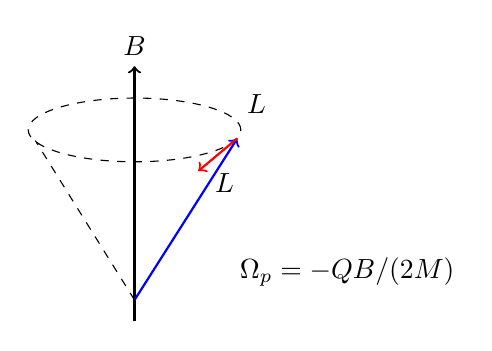
\begin{tikzpicture}[scale=.9]
\draw[->,thick](0,-.3)--(0,3.3)node[above]{$\bm B$};\draw[dashed](0,2.4)ellipse(1.5 and .45);
\draw[->,blue,thick](0,0)--(1.45,2.28);\node[above right]at(1.45,2.5){$\bm L$};\draw[->,red,thick](1.45,2.28)--(.9,1.82);\node[right]at(1,1.65){$\dd\bm L$};
\draw[dashed](0,0)--(-1.4,2.25);\node at(3,.4){$\bm\Omega_p=-Q\bm B/(2M)$};\end{tikzpicture}}
图\ref{fv:m2:precession}中角动量端点沿圆锥绕行，$\bm L\cdot\dot{\bm L}=0$保证其长度不变。由 $\bm m=(Q/2M)\bm L$得到的力矩是 $(Q/2M)\bm L\times\bm B$；要写成进动形式 $\bm\Omega_p\times\bm L$，交换叉积顺序后必须出现负号。图只示意端点的局部切向变化，进动方向还随 $Q$变号。若电荷与质量分布不成比例，或角速度不与角动量平行，就不能直接使用这一单一进动公式。


\section{短时磁冲量与机械运动的衔接}
若直棒在匀强场中受到的主要水平力为 $Bil$，即使电流随时间变化，仍可在固定方向上积分牛顿定律：
\begin{equation}m\int_{v_i}^{v_f}\dd v
=Bl\int_{t_i}^{t_f}i(t)\dd t
=Bl\int_{Q_i}^{Q_f}\dd Q
=Bl(Q_f-Q_i)=Bl\,\Delta Q.\end{equation}
因此不必先知道电流的具体时间函数，就能从速度变化反求通过的电量。成立条件是棒长、场和受力方向在积分期间不变，其他水平冲量可忽略。电流换向时，积分量是有向电荷量，不能把各时段电量的绝对值相加。


棒离轨后若电路断开，水平磁驱动力消失，后续运动可以由机械条件确定。例如从高度 $h$ 水平飞出并落地，飞行时间由竖直自由落体给出，再由水平射程确定离轨速度。将这段机械信息代回磁冲量式，就把实验可测的射程与电量联系起来。


电容放电推动导棒时，通过棒的有向电量等于电容电荷的减少量。若离轨时电容仍带电，那是切断电路时留下的状态，并不一定是整个耦合系统已达到静止或匀速的平衡态。机械冲量、电荷变化与能量是不同约束，应按所求量选取足够的方程。电磁感应专题进一步讨论动生电动势、充放电时间和热量，这里着重利用磁力积分建立机械量与电量的直接关系。


\fig{fig:mg2:k:impulse}{磁驱动段与断路后的机械运动分别建模，离轨速度由射程反求}{\begin{tikzpicture}

\begin{scope}
\draw[world](-2,.8)--(2,.8)(-2,-.8)--(2,-.8);\draw[very thick](.4,-.8)--(.4,.8);\draw[flow](.4,-.5)--(.4,.5)node[right]{$i(t)$};
\foreach \x in {-1.3,1.3}{\node at(\x,0){$\odot B$};}\draw[force](.6,1.2)--(1.9,1.2)node[midway,above]{$F_x=Bil$};
\draw[dim](-2.5,-.8)--(-2.5,.8)node[midway,left]{$l$};\node at(0,-1.6){俯视：$m\Delta v=Bl\int i\dd t$};
\end{scope}
\begin{scope}[xshift=6.6cm]
\draw[world](-1.4,1.5)--(0,1.5)--(0,-1);\draw[world](-.6,-1)--(3.1,-1);\fill(0,1.5)circle(1.7pt);
\draw[->,blue,thick](0,1.5)--(1.4,1.5)node[above]{$v_f$};\draw[dashed,domain=0:2.5]plot(\x,{1.5-.4*(\x)^2});
\draw[dim](-.8,-1)--(-.8,1.5)node[midway,left]{$h$};\draw[dim](0,-1.6)--(2.5,-1.6)node[midway,below]{$s$};\node at(.9,2.4){侧视：离轨即断路};
\end{scope}

\end{tikzpicture}}
图\ref{fig:mg2:k:impulse}左图中 $\int i\dd t$ 是通过导棒的有向电量，右图中则在电路已断开的条件下使用 $t=\sqrt{2h/g}$、$v_f=s/t$。若棒从静止开始且导轨摩擦可忽略，联立得 $\Delta Q=ms\sqrt{g/(2h)}/(Bl)$。这里先用自由飞行确定驱动结束时的速度，再对有磁力的时段积分；若飞行期间仍通电或另有水平力，右图的匀速水平运动便须相应改写。

